%!TEX root = ../../../2019main.tex
\vspace{10pt}
\subsubsection*{\bf Vibration Isolation System Type-B}
\vspace{3pt}
\noindent {\sf [Spokesperson :\ Fabian Pe\~{n}a Arellano ]}

\vspace{3pt}
\noindent {\sf \small ICRR, The Univ.\ of Tokyo, Hida, Gifu 506-1205}

\vspace{3pt}


Besides the four Type-A suspensions KAGRA relies on smaller suspensions
for other mirrors which are always at room temperature. The Type-B
suspension is used for the beam splitter and the three signal recycling
mirrors, whereas the Type-Bp is used for the three power recycling
mirrors.

\begin{figure}[h]
\begin{centering}
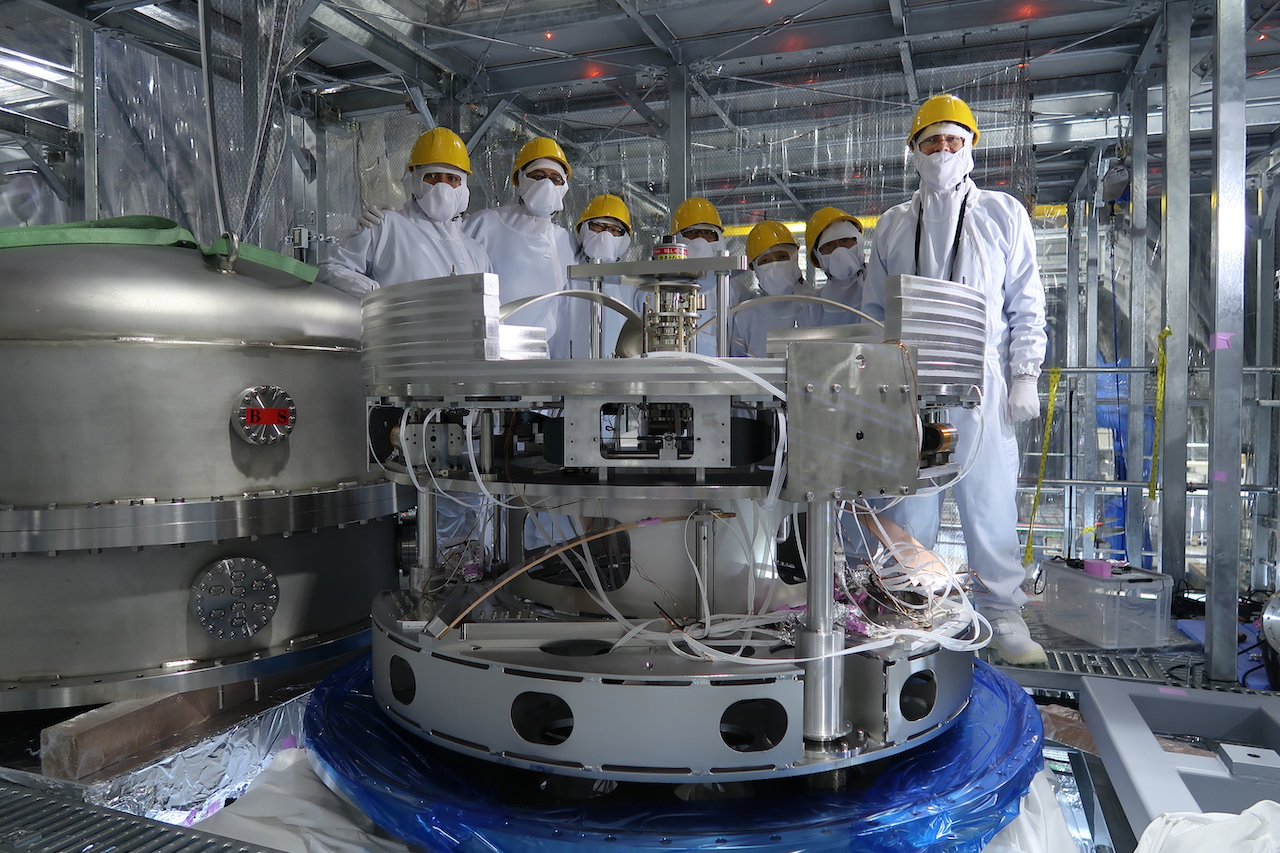
\includegraphics[width=0.48\textwidth, bb=0 0 1280 853]{astrodiv/gw/vis-b/typeB_team_01.jpg}
\par\end{centering}

\caption{The IP of the beam splitter in the vacuum chamber and the installation
team.}
\end{figure}


As in Type-A suspension, in Type-B suspension the first vibration
isolation stage is the Inverted Pendulum (IP), whose main goal is
to passively attenuate the persistent horizontal microseismic motion
produced by ocean activity. Typical resonant frequencies for these
IPs are between 60 mHz and 80 mHz in order attenuate the microseismic
peak at around 200 mHz. The following three stages, intended for vertical
isolation, are three geometric anti-spring filters. The first one
lies directly on top of the IP table while the other two hang from
it as the masses of a multi-stage pendulum. As in the case of the
IP, GAS filters are devices capable of supporting loads of hundreds
of kilograms and at the same time achieving resonant frequencies of
a few hundreds of millihertz. The horizontal position of the IP and
the vertical positions of the GAS filters are measured with Linear
Variable Differential Transformers (LVDTs) and are adjusted with coil-magnet
actuators which also damp the mechanical resonant motion. The typical
resolution of the LVDTs are below 0.2 $\mu$m. From the lowermost
GAS filter the payload hangs. The payload, which is common to Type-B
and Type-Bp suspensions, comprises the optic, its marionette and their
respective recoil masses. The recoil mass of the marionette holds
local displacement sensors to monitor six degrees of freedom and coil-magnet
actuators for damping the resonant modes of oscillation of the suspension
itself. The sensors have typical resolutions of about 20 nm. The recoil
mass of the mirror holds coil-magnet actuators only and the system
relies on an optical lever to monitor the tilt and position of the
optic from the ground.

The Type-Bp suspension is shorter and comprises two GAS filters and
the payload. The uppermost GAS filter lies directly on the ground
while the lowermost one has its own recoil mass in order to attenuate
motion which may be excited by the microseismic motion of the ground.